\documentclass{article}

\usepackage{fullpage}
\usepackage{amsmath}
\usepackage{amssymb}
\usepackage{graphicx} 
% \marginparwidth = 35pt
\usepackage[norsk]{babel}              % norske navn rundt omkring
\usepackage[T1]{fontenc}              % gir tilgang til alle tegn i fonten
\usepackage[utf8]{inputenc}         % utf8 rules them ALL
\usepackage{parskip}
\usepackage{multirow}
\usepackage{listings}
\usepackage[table]{xcolor}
\usepackage{fancyhdr}
\usepackage{hyperref}

% forside 
\newcommand{\PageTitle}{Detaljert Brukermanual}
\newcommand{\DateDeadline}{\today}

% SAKSMACRO
\newcommand{\sak}[2]{\section*{Sak #1: #2}}

% Bildemakro 
\def\imagetop#1{\vtop{\null\hbox{#1}}}



\begin{document}
% Importert fra fil 
\newcommand{\HRule}{\rule{\linewidth}{0.5mm}}
\begin{titlepage}
	\vspace*{3cm}
	\begin{center}
		{\Large RMI med prosjekt i distribuerte systemer TDAT3014}
		\HRule \\[0.5cm]
		{\LARGE\textsc{\textbf{\PageTitle}}}
		\HRule \\[1.0cm]
		{\large \DateDeadline} 
		\vspace{\fill}
		\begin{flushleft}
		\emph{Gruppemedlemmer}:\\
			{Andreas Mosti, \ Thomas Mowatt} 
		\end{flushleft}
	\end{center}
\end{titlepage}



\newpage
.\vfill
\begin{centering}
\LARGE


\textit{Et dokument om}  \\ 
\ \textit {Simple Network Server -} \\ 
\ \textit {Produktet}
\vspace{12cm}
\hspace{15cm}
\newpage
\end{centering} 
\fancyhead[L]{
Simple Network Server		\hfill			 Version: 1.1 \\
Detaljert Brukermanual 	\hfill			Date: \today  \\}
\pagestyle{fancy}
\setlength\headsep{30pt}


\begin{table}[h] % http://en.wikibooks.org/wiki/LaTeX/Tables

\caption{Revisjonshistorikk}
	\begin{tabular}{| m{3cm} | m{1cm} | m{5cm} | m{4cm} |} 
	\hline	
	Dato & Versjon & Beskrivelse & Forfatter\\ 
	\hline
	 25/01/14 & 1.0 & Første versjon ferdigstilt & Andreas Mosti og Thomas Mowatt\\ 
	\hline
	25/01/14 & 1.1  & Rettskrivning og revisjon  & Andreas Mosti og Thomas Mowatt \\ 
	\hline
	 &  &  & \\ 
	\hline
	
	\end{tabular}
\end{table}

\newpage

\tableofcontents
\newpage
\section{Introduksjon}
\subsection{Mål}
Dette dokumentet er ment som brukermanual for Simple Network Server - produktet. Det vil inneholde alt som trengs for å kunne bruke løsningen fullt ut, inkludert avhengigheter og oppsett.
\subsection{Omfang}
Dette dokumentet omhandler bruk av hele systemet. \\ Beskrevet miljø er Linux (Debian - basert) og Mac OS X 10.9.
\\ MERK: Prosjektet er tilgjengelig for Windows, men dette er ikke testet. 
\subsection{Definisjoner, akronymer, forkortelser}
\begin{itemize}
\item SNS: Simple Network Server
\item SSH: Secure Shell
\item OS: Operating System
\item LAMP: Linux Apache MySql PHP
\item ISP: Internet Service Provider
\item IPS: Intrusion Preventning System
\item DDOS: Distributed Denial-Of-Service
\item NAT: Network Address Translation
\end{itemize}
\\
\subsection{Referanser}
\begin{itemize}
\item{Mitchell Hashimoto, Vagrant: Up and Running}
\item Visjonsdokument, Kravdokument og Arkitekturdokument
\item Se fotnoter
\end{itemize}
\subsection{Innholdsoversikt}
\section{Kort om Simple Network Server}
Simple Network Server (SNS) er et ferdig, utvidbart virtuelt servermiljø basert på Ubuntu Linux som inneholder programmvare og verktøy tilpasset faget LV473D -Nettverkssikkerhet. Systemet er ment for kjapp installasjon av et ferdig servermiljø basert på verktøyene Vagrant og Virtualbox. Versjon 1.0 er ment som et rammeoppsett med grunnnfunksjonalitet, selv om videre utvidelse anbefales etter behov.
\section{Testoppsett}
Denne manualen er skrevet ut ifra gjennomgang og bruk på våre testoppsett og fungerer 100\%. Disse er idag: 
\begin{itemize}
\item MacBook Pro Retina 13'', OS X  ''Maverics'' 10.9.1, 64 bit
\item Debian ''Wheezy'' 3.2.51-1, 64 bit
\item Ubuntu ''Precise Pangolin'' 12.04LTS, 32 bit
\item Ubuntu ''Precise Pangolin'' 12.04LTS, 64 bit
\item Ubuntu ''Saucy Salamander' 13.10, 64 bit
\end{itemize}
\section{Installasjon og grunnnoppsett}
For å ta i bruk Simple Network Server - oppsettet for første gang må man først installere to avhengigheter samt hente ned prosjektet. Vi begynner programvare som kreves:
\subsection{Virtualbox}
Siden SNS bygges opp rundt en virtuell server, må virtualiseringsløsningen virtualbox tas i bruk. Virtualbox er gratis, og kan lastes ned via \url{https://www.virtualbox.org/wiki/Download_Old_Builds} for Linux og Mac. Pakken kan også lastes rett fra pakkerepoet til Debian / Ubuntu: \\ 
\begin{lstlisting}
sudo apt-get install virtualbox
\end{lstlisting}
\\
Eller via macports\footnote{https://www.macports.org/} på OS X:
\begin{lstlisting}
sudo port install virtualbox
\end{lstlisting}
\\
Testet og anbefalt versjon er virtualbox 4.1.18. 
\subsection{Vagrant}
Den neste nødvendige programmvaren er Vagrant. Vagrant er det virtuelle miljøet SNS benytter for å kjøre, og er ment for å lage virtuelle utviklermiljøer som fokuserer på å skape identiske maskinoppsett for alle som jobber på et delt prosjekt. Ved bruk av Vagrant vil prosjektet oppføre seg likt for alle som tar det i bruk. Som utviklerne av Vagrant selv beskriver det: 
\begin{quote}
''Vagrant is a tool for building complete development environments. With an easy-to-use workflow and focus on automation, Vagrant lowers development environment setup time, increases development/production parity, and makes the ''works on my machine'' excuse a relic of the past.''\footnote{\url{https://www.vagrantup.com/about.html}}
\end{quote}
For å installere Vagrant, last ned fra \url{http://downloads.vagrantup.com} for Linux og Mac. \\
 Pakken kan også lastes rett fra pakkerepoet til Debian / Ubuntu: \\ 
\begin{lstlisting}
sudo apt-get install vagrant
\end{lstlisting}
\\
Eller via macports på OS X:
\begin{lstlisting}
sudo port install vagrant
\end{lstlisting}
\\
Testet og anbefalt versjon av vagrant er 1.2.7. 
\footnote{Vagrant: Up and Running av vagrantskaper Mitchell Hashimoto kan eventuelt brukes som støttelitteratur. }

\subsection{Kildekode}
Selve kildekoden til SNS hentes fra github for enklest installasjon: 

\begin{lstlisting}
git clone https://github.com/andmos/SNS
\end{lstlisting}
\\
Nå kjøres prosjektet for første gang enkelt ved å skrive følgene i kommandolinja: 
\begin{lstlisting}
cd SNS/
vagrant up
\end{lstlisting}
\\ \\
Et virtuelt Ubuntu - image vil nå lastes ned (skjer kun ved første gangs kjøring) og prosjektfilene vil settes opp på dette imaget. 
Skjermbildet ved første gangs innhenting av image ser slik ut: \\ \\
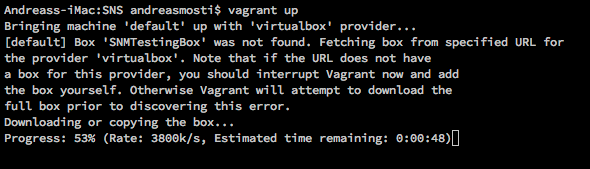
\includegraphics[scale = 0.7]{pictures/vagrantFirstTime.png}
\\ \\
Dette imaget er det vagrant kaller en ''box''. Den fungerer som grunnnimage, og nedlastning skjer som sagt kun ved første gangs bygg av prosjektet. Ved alle nyoppsett av systemet vil imaget brukes som grunnn-OS for prosjektfilene til SNS, eller en såkalt ''sandbox''. Boksen kan lokaliseres i den skjulte mappa ''./vagrant.d'' på hjemmekatalogen til brukeren din. \\ \\
For å sjekke at den virtuelle maskinen fungerer som den skal, gå til \url{http://localhost:8080/} fra nettleseren din. Du vil da få opp denne siden:
\\ \\
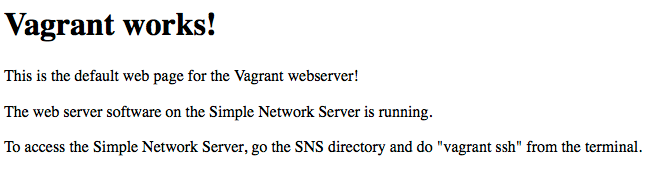
\includegraphics[scale = 0.7]{pictures/vagrantWorks.png} 
\\ \\

\subsection{Kjente oppsettsproblemer}
Den eneste feilen som har oppstått under testing er at versjonene av Virtualbox og Vagrant som ligger i repoene har vært ikke-kompatible med hverandre. Skulle dette oppstå ved oppsett, må man manuelt laste ned Virtualbox versjon 4.1.18 og legge denne inn. For 32 bit: 
\begin{lstlisting}
wget http://download.virtualbox.org/virtualbox/4.1.18/
virtualbox-4.1_4.1.18-78361~Ubuntu~precise_i386.deb
sudo dpkg -i virtualbox-4.1_4.1.18-78361~Ubuntu~precise_i386.deb
\end{lstlisting}
Og for 64 bit:
\\ 
\begin{lstlisting}
wget http://download.virtualbox.org/virtualbox/4.1.18/
virtualbox-4.1_4.1.18-78361~Ubuntu~precise_amd64.deb
sudo dpkg -i virtualbox-4.1_4.1.18-78361~Ubuntu~precise_amd64.deb
\end{lstlisting}
\\ 
Merk: Dette er pakker for Ubuntu 12.04 LTS. For andre versjoner av OS X / Linux, last ned fra \\
\url{https://www.virtualbox.org/wiki/Download_Old_Builds_4_1}
\\ \\ \\
Skulle problemer med Vagrant oppstå, kan også denne installeres utenom pakkesystemet. Da kjøres følgende (32 bit): 
\begin{lstlisting}
wget http://files.vagrantup.com/packages/7ec0ee1d00a916f80b109a298bab08e391945243/
vagrant_1.2.7_i686.deb 
sudo dpkg -i vagrant_1.2.7_i686.deb 
\end{lstlisting}
\\
Og for 64 bit - versjonen: 
\begin{lstlisting}
wget http://files.vagrantup.com/packages/7ec0ee1d00a916f80b109a298bab08e391945243/
vagrant_1.2.7_x86_64.deb
sudo dpkg -i vagrant_1.2.7_x86_64.deb
\end{lstlisting}
\\ 
Igjen, dette er pakker for Ubuntu. For andre distroer og OS X, besøk \\
\url{https://downloads.vagrantup.com/tags/v1.2.7} \\ \\
Erfaringer under testing har knyttet kjente problemer opp mot Virtualbox, så begynn med den.
\section{Arbeidsflyt}
Arbeidsflyten for produktet er veldig enkel. Når man står i prosjektets mappe, startes den virtuelle maskinen enkelt ved \\
\begin{lstlisting}
vagrant up
\end{lstlisting}
\\ 
Og maskinen aksesseres via SSH ved
\begin{lstlisting}
vagrant ssh
\end{lstlisting}
\\
Man blir da møtt av følgende skjermbilde: \\ \\
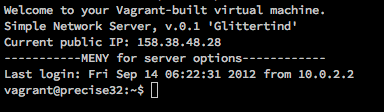
\includegraphics[scale = 0.7]{pictures/vagrantSSH.png}
\\ \\
og kan nå bruke alle verktøyene SNS tilbyr enkelt via kommandolinja, hovedsaklig via ''meny'' kommandoen for enkelhets skyld. Det er verdt å merke seg at SNS - maskinen er en fullverdig virtuell Ubuntu - maskin, så all Linux - funksjonalitet utenfor prosjektets verktøy kan fritt brukes og / eller installeres. \\ 
Når man er ferdig med maskinen, avslutter man SSH - sesjonen og skriver: \\
\begin{lstlisting}
vagrant destroy
\end{lstlisting}
\\
Alle endringer og oppsett på den virtuelle maskinen blir nå slettet. Har man foreks. rotet det til med filer, angrepet serveren slik at den ikke lengre kan brukes fullstendig eller liknende, er ikke det noe problem. Nåværende system slettes. For neste gangs bruk av SNS, kjører man enkelt og greit ''vagrant up'' igjen, og prosjektet settes opp på nytt fra bunn av. Gjennomsnittlig oppstartstid på en Macbook Pro med 8 Gb minne, Intel i5 2.5Ghz og SSD disk på skolens linje er på 4 minutter og 45 sekunder, noe som må sies å være meget bra for et system som installerer programmvare fra bunn av ved oppkjøring.
\section{Gjennomgang av nåværende funksjonalitet}
For å benytte seg av funksjonaliteten som er bygget inn i SNS har vi laget en oppstartsmeny som enkelt og greit skal kunne guide deg til den funksjonaliteten du er ute etter (se kravdok). Du kommer til denne menyen når SNS er startet, og ''vagrant ssh'' er kjørt. Ved så å skrive ''meny'' fra kommandolinja, blir man møtt av følgende vindu: 
\\ \\
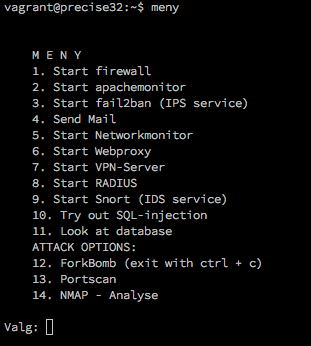
\includegraphics[scale=0.8]{pictures/meny.png} 
\\ \\
I dette avsnittet går vi gjennom hver av disse valgene, med forslag til bruk og utvidelse. 
\subsection{1: Start firewall}
Det første valget starter et skript som er tilpassed demonostrasjon av brannmur. \\ Her er funksjonaliteten ganske enkel: et skript starte brannmurprogrammvaren (ufw, abstraksjonslag oppå iptables) og laster inn en på forhånd oppsatt konfigurasjon som låser ned serveren, med unntak av portene som aktivt brukes i SNS som åpnes. Når skriptet er ferdig, dukker en oversikt over de åpne portene opp. 
\\ \\
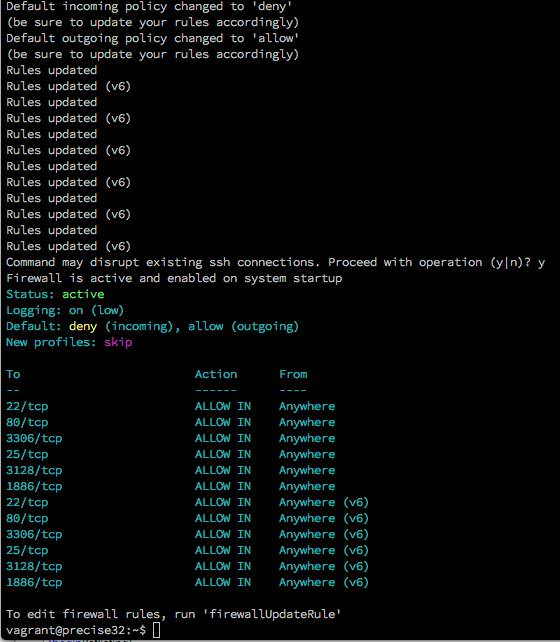
\includegraphics[scale = 0.7]{pictures/firewall.png}
\\ \\ 
Som vi ser av bildet, er de portene som er markert som åpne inn kun de som er i bruk av Simple Network Server. 
For å demonstrere brannmurendringern, kan skriptet 'firewallUpdateRule' kjøres rett fra kommandolinja. Dette skriptet er skrevet for enkelt og greit å gjøre endringer i aksesspolicyen til portene på serveren. Du velger om en port skal åpnes eller lukkes, og får da ny oversikt over portene på serveren. Dette for å lett kunne demonstrere brannmurens virkemåte. Eksempel på bruk kan være å stenge port 80, for så å besøke \url{http://localhost:8080} og se at aksessen nå er sperret. Annen bruk kan være å kjøre portscanner mot serverens adresse og se på åpne porter. 
\\ \\ 
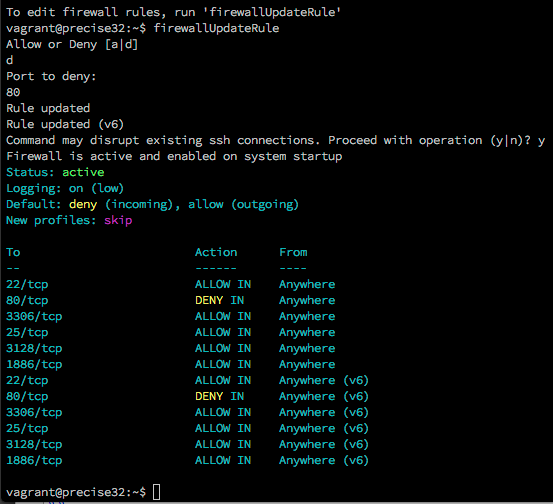
\includegraphics[scale =0.7]{pictures/firewallUpdate.png}
\\ \\
Eksempel på bruk av 'firewallUpdateRule', port 80 blir sperret.
\subsection{2: Start apachemonitor} 
Dette valget er ganske rett fram; et tilpasset skript deler skjermen i to og viser henholdsvis error og standard - loggen til webserveren apache2. Dette for å vise oppføringer som kommer når vi besøker sider hostet på webtjeneren, og kan vise hva som skjer når vi bestemmer oss for å ''plage'' LAMP - serveren.
\\ \\
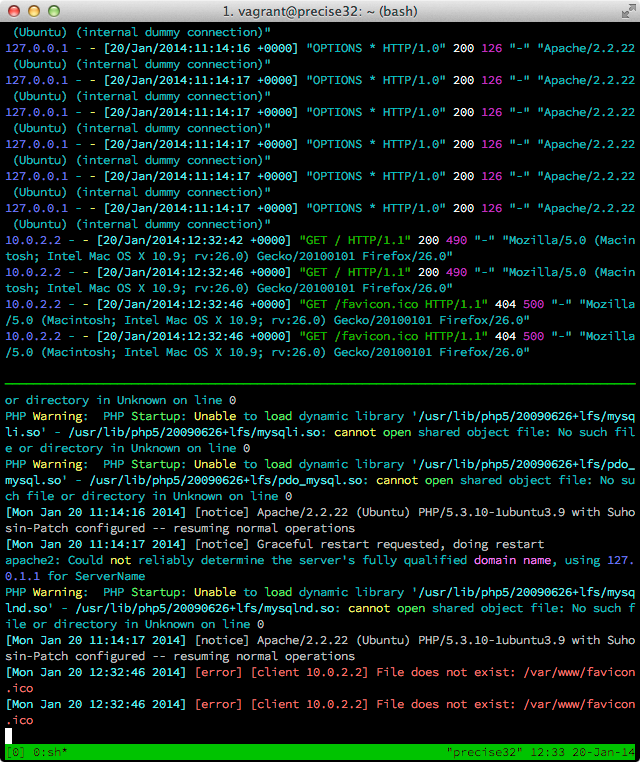
\includegraphics[scale= 0.7]{pictures/apachelogg.png}
\\ \\
Bildet viser eksempel på loggoppføring ved vanlig besøk på innhold hostet av webtjeneren. Leg merke til advarsel om fil som ikke eksisterer, denne feilen er framprovosert for å vise feil i loggen. Eksempel på bruk kan være å se hva som skjer i loggen om en modifisert get - request blir sendt. 
\subsection{3: Start fail2ban (IPS Service)}
En av de mest effektive Intrusion Prevention System - tjenestene der ute er fail2ban. Den banner rett og slett IP - adresser som prøver seg på bruteforce - angrep på serveren. Tjenesten starter fail2ban etter en gitt tid. For å demonstrere bruk av fail2ban kan python-skriptet ''ssh\_forcer.py'' kjøres fra host - maskinen. Skriptet ligger på ''SNS/bin/Client/ssh\_forcer.py''. Skriptet trenger noen pakker for python, som kan skaffes ved å kjøre ''SNS/bin/pythonDependencies''. Skriptet vil prøve å brutforce SSH - login på SSN - serveren, passordforsøk på passordforsøk. Ved å aktivere fail2ban, kan man se at angrepsforsøkene stopper fordi IPen til slutt blir bannet. Effektiv demo av en IPS sine egenskaper: Den gjør aktive tiltak mot angriper.
\\ \\
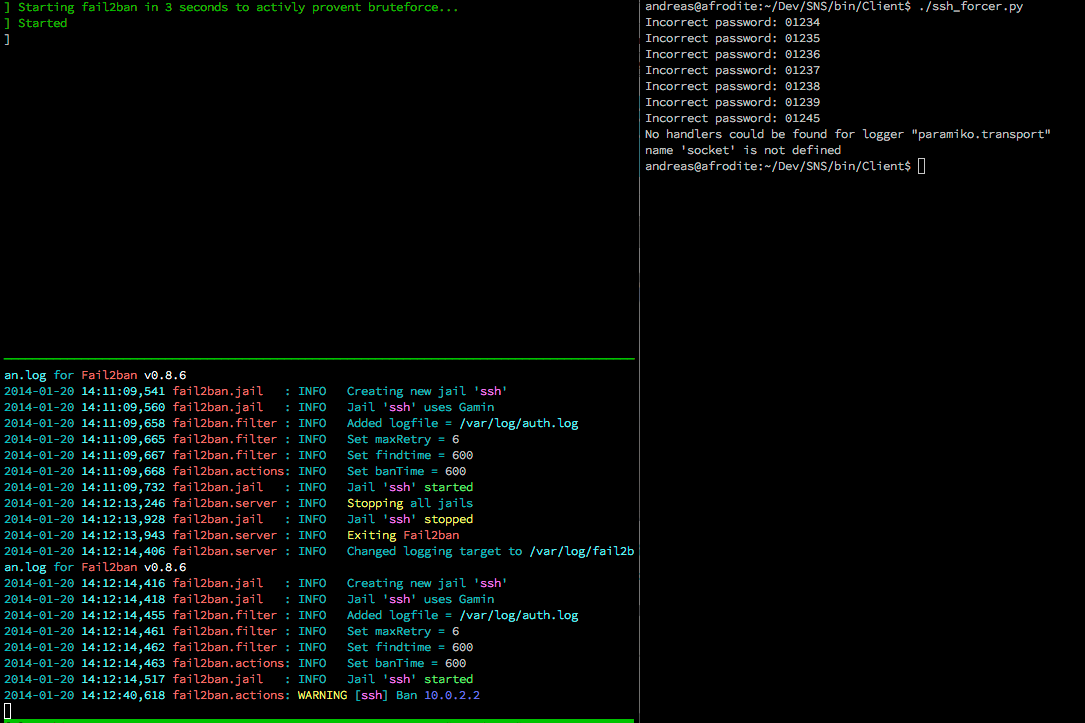
\includegraphics[scale = 0.5]{pictures/ips.png}
\\ \\
Bildet viser bruk av ssh\_forcer og IPS - pakken. Her får angriper prøvd seg 7 ganger før fail2ban starter og får sendt IPen i ''fengsel''. Utvidelse her kan være bruteforce - forsøk på HTTP - serveren. 
\subsection{4: Send mail}
Dette valget er ment som en demonstrasjon av hvor enkelt det er å sende epost med falsk avsender, som igjen kan føre til både phishingforsøk og spam. I dag regnes hele 80 - 85 \% av all mailtrafikk som spam.\footnote{Kilde: https://en.wikipedia.org/wiki/Spam_\%28electronic\%29#cite_note-4} Skriptet som starter mailsendingen spør deg om mottakeradresse (NB: ikke benytt skriptet uten at mottaker er klar over det!) og en ønsket avsenderadresses. Etter noen sekunder sendes mailen ut fra serveren, med en standard tekst som ligger lagret på ''/SNS/resources/doc/MailMessage''. \\ OBS: For at denne funksjonaliteten skal funke kan man \textit{ikke} være bak brannmur som stopper trafikk på SMTP - porten. Vanlige ISPer som Canal Digital osv. stopper trafikk her. Dette er derimot ikke et problem på HiST, hvor SNS hovedsaklig skal brukes. 
\\ \\
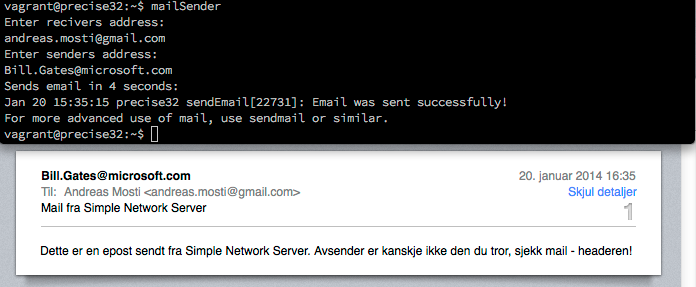
\includegraphics[scale = 0.7]{pictures/mailsender.png}
\\ \\ 
Her ser vi bruk av mailsender, hvor Bill Gates tilsynelatende har sendt mail. Men, som teksten sier, burde man sjekke mailheaderen for å se om avsender er den han er. Videre bruk av tjenesten kan være å lage til en phising - mal som sendes, for å demonstrere hvor enkelt det er å lage en tilsynelatende ekte mail fra foreks. banken din. Et annet bruksmønster er å overvåke pakkene som går; tjenesten er lagt opp til å sende mail uten kryptering, så alt går i klartekst. Dette er også grunnnen til at mailen venter 4 sekunder før den sendes, så foreks. Wireshark kan rettes mot serverens IP for se på pakkene som går. 
\subsection{5: Start networkmonitor}
Dette valget er en nettverksmonitor satt sammen av programmene Nethogs og Iftop. Nethogs viser hvilke kjørende prosesser som genererer nettverkstrafikk, både innkommende og utgående, mens Iftop viser trafikk på eth0 - kortet, altså nettverkskortet på serveren. iftop viser hvilke IPer som blir kommunisert med, og hvor mye trafikk som går. Fordi SNS er bygget opp fra grunn av med \textit{kun} den funksjonaliteten vi ønsker for å demonstrere forskjellige aspekter ved faget Nettverkssikkerhet, vil det være få prosesser som kjører (SNS er programmert til å blokkere alle tjenestene fra oppstart, de blir kun aktive når du velge å bruke dem) som igjen fører til en ren og ryddig logg: den blir ikke oversvømt av prosesser som bruker nettverk. Dette verktøyet er derfor veldig fint å bruke for å demonstrere hvordan prosesser bruker trafikk inn / ut av serveren. 
\\ \\
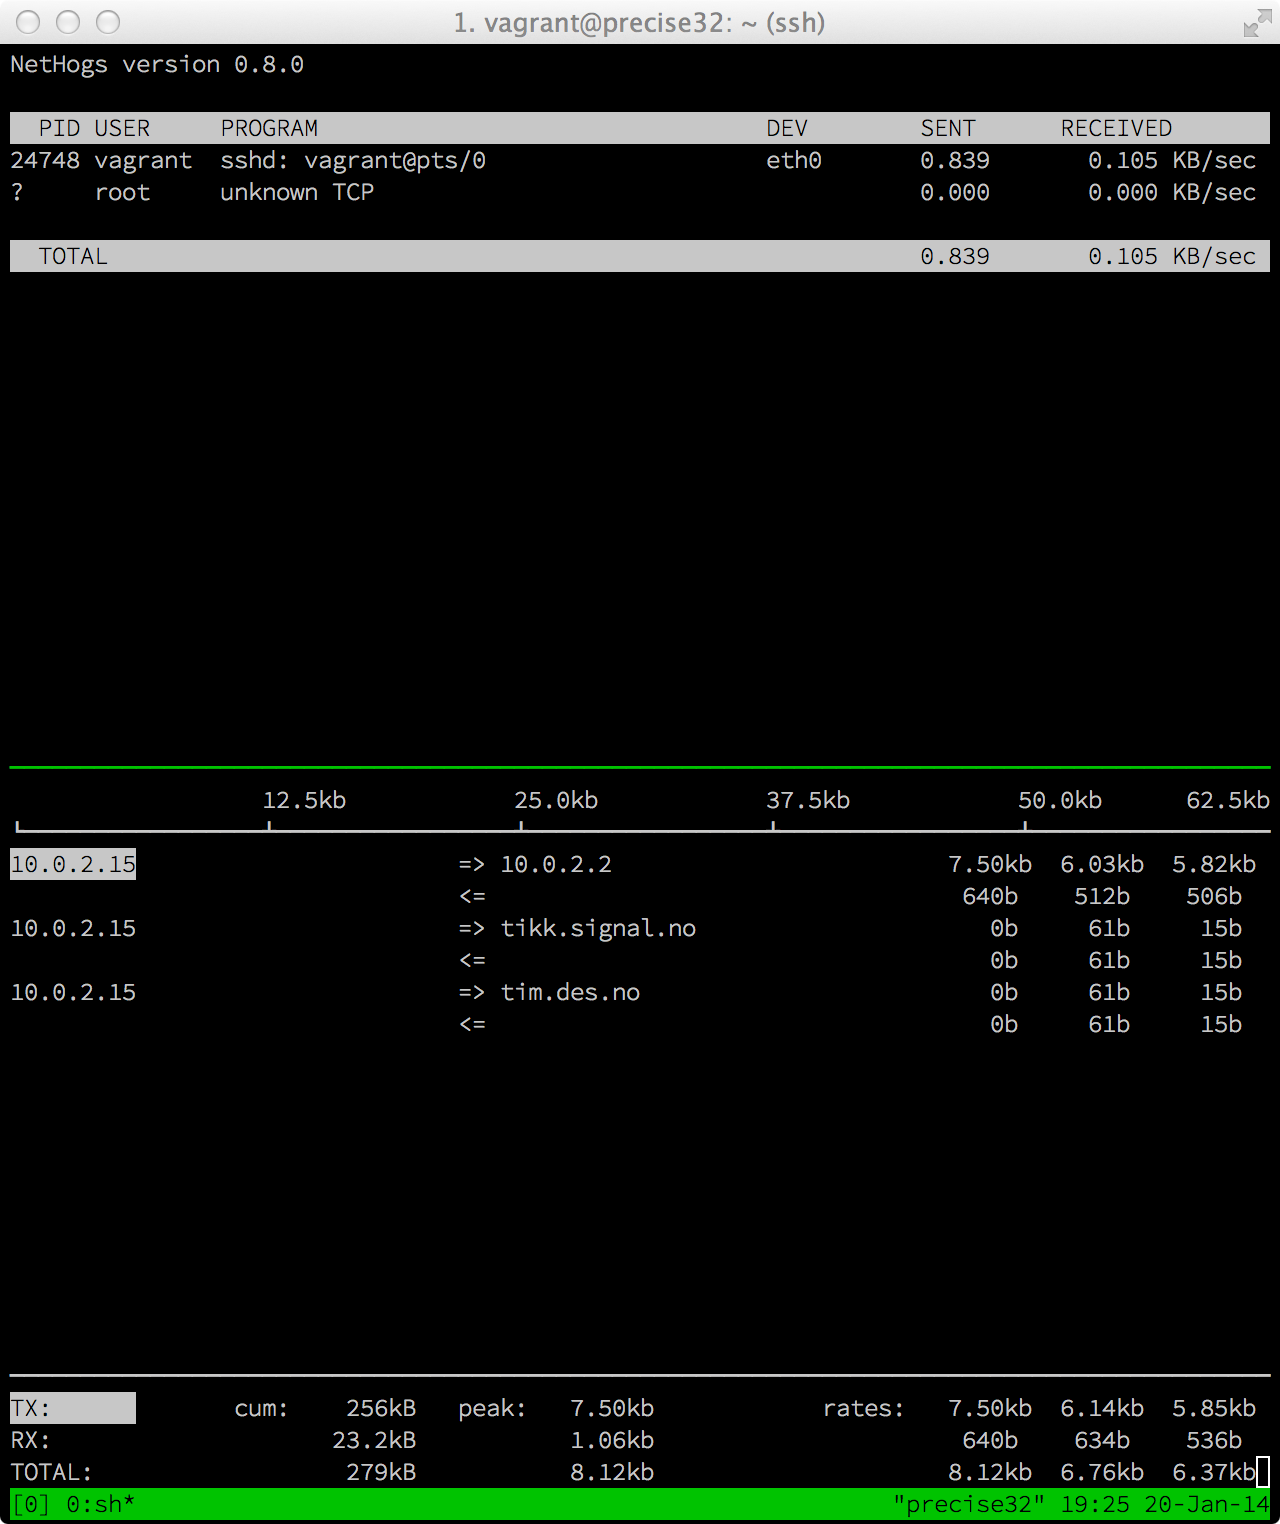
\includegraphics[scale = 0.6]{pictures/networkmonitor.png} 
\\ \\
Det øverste vinduet er Nethogs, som her kun viser en aktiv prosess som bruker av nettverket, nemmlig SSH, som jeg kommuniserer med serveren via. \\ 
Nedenfor ser vi iftop som melder om trafikk fra serveren til 10.0.2.2 som er hostmaskinens IP, samt trafikk til Signal, som er ISP der serveren står.
Forslag bruk av denne nettverksmonitoren er som nevnt å vise hvordan trafikk til / fra serveren vises, og man kan demonstrere hvor greit det er å holde orden på hvilke prosesser som bruker nettverksresurser i systemet. Skulle serveren bli kompromitert og bli en del av et botnet, kan man da helt klart se av monitoren om noe genererer mye trafikk. 
\subsection{6: Start webproxy}
For å demonstrere hvordan webtrafikk kan dirigeres gjennom en proxy, har vi satt opp en egen tjeneste basert på webproxyen squid3. Når denne tjenesten starter, får man opp en todelt skjerm: den øverste delen viser informasjon om adresse og port til proxyen, samt informasjon om blokkede nettsider. Man kan enkelt benytte denne proxyen fra klientmaskinene på samme nett, ved å konfigurere nettleseren din. Å bruke webproxy er en fin måte for arbeidsgivere å kontrollere hvilke nettsider som besøkes, samt blokke uønskede tidstyver som facebook. Den andre delen av skjermen viser loggen til proxyen, med informasjon om hvem som har besøkt hvilke sider. \\
For å angi andre blokkede sider, rediger følgende fil: ''/SNS/resources/squidRules/blockedSites''. I ''squidRules'' - mappa ligger også konfigurasjonsfilen til proxytjenesten.
\\ \\
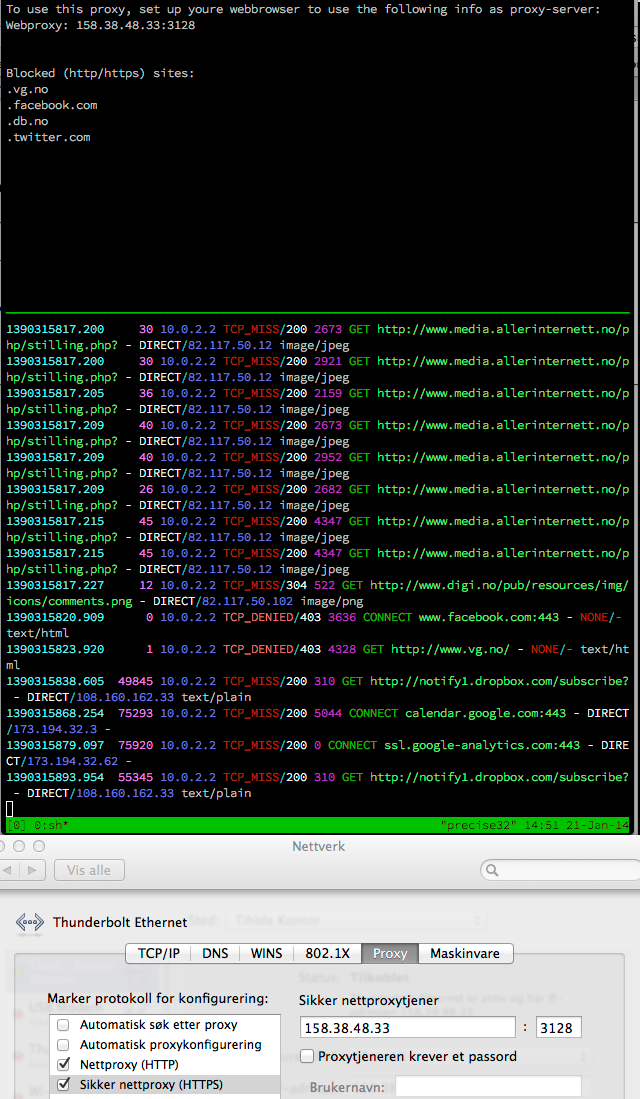
\includegraphics[scale = 0.5]{pictures/proxy.png}
\\ \\
På bildet ser vi tjenesten i aksjon. Neders er en maskin med OS X konfigurert til å bruke webproxyen vår, og loggen viser trafikk mot blant annet digi.no, mens trafikk rettet mot vg.no blir blokkert. 
\subsection{7: Start VPN-Server}
En nettverksfunksjonalitet som er inn for tiden er VPN. Med VPN får man opprettet en kryptert tunell inn mot en server, slik at man får tilgang til resurser på denne, eller nettet den er knyttet opp mot. For å demonstrere dette har vi satt opp en av de mest brukte VPN - tjenerne, OpenVPN AS (AS står i dette tilfelelt for access - server.) Når valget er tatt, kommer det opp informasjon om tilkobling. Vi har gått for en enkel løsning her, så vinduet ser slik ut: 
\\
\\
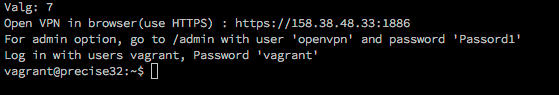
\includegraphics[scale = 0.7]{pictures/vpn.png}
\\ 
\\
Oppgitt URL leder til tilkoblingsside som laster ned klient til det OSet du sitter på, og lar deg automatisk koble opp mot serveren vår.
Skulle det være ønskelig med demonstrasjon av adminpanelet til openvpn, kan dette gjøre via /admin - siden. 
\\
\\

\includegraphics[scale = 0.7]{pictures/vpn2.png}
\\ 
\\
Bildet over vise videresending ved login på VPN - tjeneren.
\subsection{8: Start RADIUS}
RADIUS er en fin måte å sentralisere administrasjon av nettverkskomponenter, da særlig brukernavn / passord for switcher, rutere osv. Vanligvis koblet RADIUS opp mot en katalogtjeneste (som foreks. LDAP eller Actitve Directory), men fordi vår løsning skal være så lettvektig som mulig har vi ikke satt opp noen LDAP som en del av tjenesten. Vi har derimot laget rammeverket klart, samt en liten demonstrasjon av en bruker som får autentisert seg mot RADIUS:
\\ 
\\
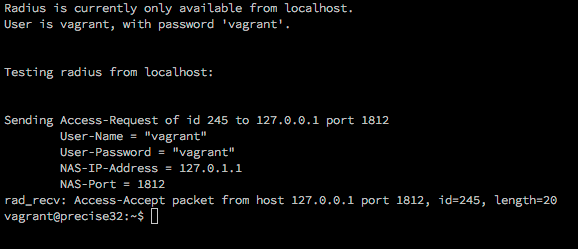
\includegraphics[scale = 0.7]{pictures/radius.png}
\\ 
\\
Foreslått videreutvikling her kan være å legge til flere brukere og åpne for tilkobling utenfor eget nett for demonstrasjon.
\subsection{9: Start Snort (IDS service)}
En av de nyttigste verktøyene i nettverksmonitoreringskassa er et Intrusion Detection System, IDS. Et IDS analyserer trafikken som går i nettet, kjenner igjen mønstre og varsler om ting som kanskje ikke er som det skal være: Portscanning, forsøk på DDOS osv. blir identifisert og varslet om. SNS kommer med en ferdigkonfigurert Snort - løsning, som monitorerer det virtuelle nettverkskortet sitt.
\\
\\
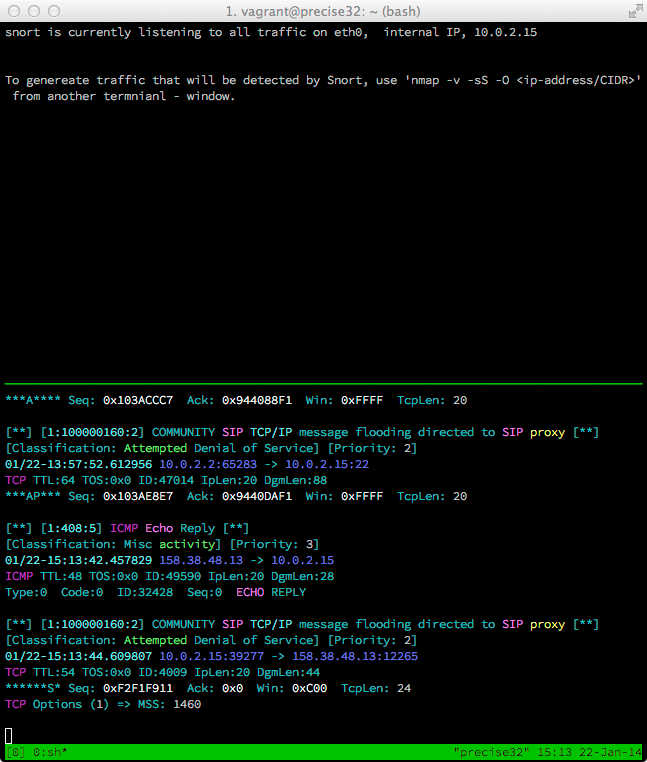
\includegraphics[scale = 0.7]{pictures/snort.png}
\\
\\
Bildet over viser Snort skriptet vårt under bruk. Her kjøres en nettverkskartlegging via NMAP ut fra serveren, og Snort varsler om at trafikken kan være en del av et DDOS - angrep, samt at porter blir scannet. Regelsett for Snort lastes inn fra ''/SNS/resources/snortRules'', så en utvidelse med nye regler kan fint legges i denne mappa, og de vil da automatisk bli lagt inn til Snort ved oppstart av SNS. Ellers står man fritt til å bruke forskjellige angrepsteknikker mot serveren, for å se hvordan systemet ser ut. 
\subsection{10: Try out SQL - injection}
Et potensielt stort sikkerhetsproblem i nett er dårlig oppsatte / programmerte webtjenere. For å demonstrere dette har vi satt sammen en MySQL - database med ''kontoer'', og en frontend skrevet i PHP. Denne siden er ment som eksempel på en enkel nettbank: Du logger deg inn med brukernavn og passord, og får tilgang til kontoopplysningene dine, som ligger i databasen. For å demonstrere dårlig skrevet kode, har vi bevisst laget login - formen uten å sikre siden mot SQL - injections. 
\\
\\
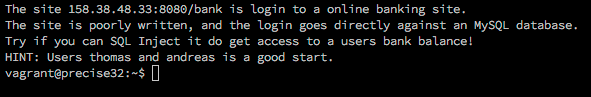
\includegraphics[scale = 0.8]{pictures/sqlinject.png}
\\
\\
Bildet over viser infoen som kommer på skjermen, mens bildet under viser loginskjermen.
\\
\\
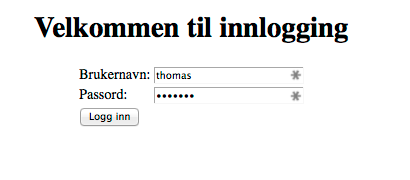
\includegraphics[scale = 0.7]{pictures/bank.png}
\\
\\
Brukernavn og passord ligger i databasen, men her ønsker vi at folk skal prøve å ''hacke'' seg inn på siden ved hjelp av SQL - injection. 
Når man prøver seg fram, vil SQL - spørringen som blir sendt inn presentert på skjermen, som en liten hjelper. \\ 
Et forslag til løsning er å sende inn ''thomas'-- '' og hva som helst som passord. Da blir SQL settningen seende slik ut: 
\begin{lstlisting}
SELECT * FROM konto WHERE kontoeier = 'thomas'-- ' AND passord= 'pass' 
\end{lstlisting}
\\ 
Forslag til bruk er å ha en konkurranse blant elevene i forelesningen, om hvem som klarer å bryte seg inn kjappest. 
\subsection{11: Look at database}
Denne funksjonen er ment som en utvidelse av SQL-Inject - funksjonen. Det eneste den gjør er å mappe ut ''Konto'' tabellen, med brukernavn, passord og saldo. Kan brukes som fasit, eller bare for å se på basen. Alle SQL - filene ligger lagret på ''/SNS/resources/databases'', og blir lastet inn til MySQL - basen ved oppstart. Man kan derfor fritt legge til flere databaser for import her.
\subsection{12: ForkBomb (exit with ctrl + c)}
Nå er vi over på et par angresskript som er skrevet som eksempler til prosjektet. ForkBomben viser hva som skjer om en bruker på en Linux - server ikke har begrensninger på hvor mange prosesser han kan kjøre, noe som kan demonstrere en dårlig oppsatt terminalserver. ForkBomben er meget enkel: 
\begin{lstlisting}
#! /usr/bin/perl
# Careful about this, use only if you know what you are doing
my $count = 0;
while(1) {
    fork();
    print $count;
    $count++;
}
\end{lstlisting}
Skriptet genererer rett og slett en ny prosess for hver gjennomgang, altså n for hver gjennomkjøring. Over litt tid blir dette veldig mange prosesser, noe som sløver ned serveren til det ubrukelige, og er ment som eksempel på sikkerhetshull. 
\\
\\
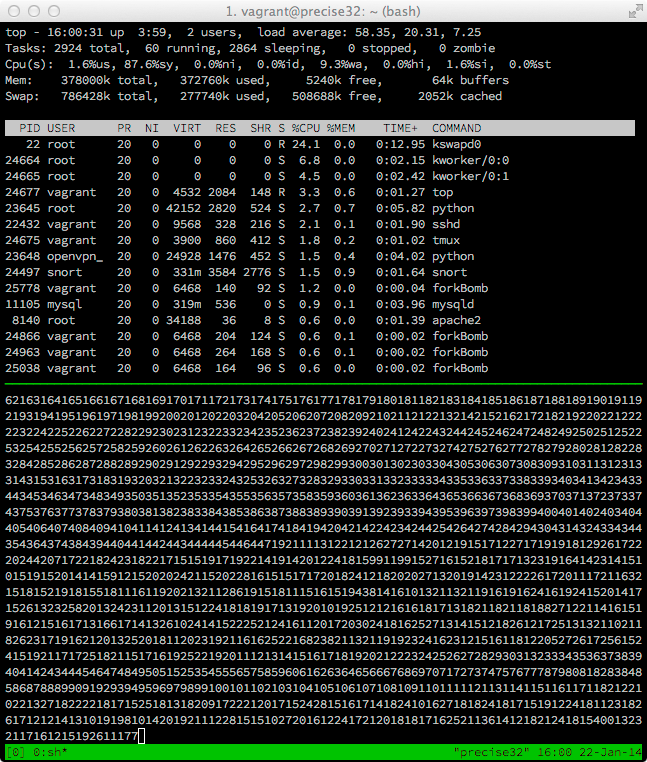
\includegraphics[scale = 0.6]{pictures/forkbomb.png}
\\
\\
Bildet viser kjøring av ForkBomb, som her bruker 87\% CPU, og har til nå generert 2924 prosesser. 
\subsection{13 og 14: Portscan og NMAP - analyse}
De to siste funksjonene er script som kjører NMAP og portscan - analyse av serveren, rett og slett for å vise hvor kraftig NMAP er. 
Selve angrepsdelen av prosjektet kan godt bygges på med flere skript.
\end{lstlisting}
\section{Om kildekodens oppbyggning}
For å forstå hvordan Simple Network Server fungerer og for å gjøre en utvidelse lettere, følger denne beskrivelsen av kildekoden. Her presenteres de viktigste elementene, mappe for mappe. Selve rota i prosjektmappa ser slik ut:  
\\
\\

\includegraphics[scale = 0.580]{pictures/struktur.png}
\\ 
\\
\subsection{Rotkatalogen}
De viktigste filene på rota er ''Vagrantfile'' og ''freshInstallWeb''.
Vagrantfile er selve ''oppskriften'' på hvordan prosjektet skal settes opp. Den gir instrukser til den virtuelle serveren som kjører i Virtualbox, på hvordan kommandoer som skal kjøres ved oppsett, samt hvilke porter som skal sendes hvor (den virtuelle maskinen er koblet til nettverket ved hjelp av NAT fra hovedmaskinen den kjører på). Kort fortalt, Vagrantfila er den viktigste fila i prosjektet, selve ''byggfila'' som starter prosjektet. Er ikke vagrantfila tilstede, går det ikke ann å kjøre ''vagrant up'' kommandoen. 
\\ \\
\newpage
Vi tar en nærmere titt på fila:
\begin{lstlisting}
# -*- mode: ruby -*-
# vi: set ft=ruby :

Vagrant::Config.run do |config|
  config.vm.box = "Simple Network Server box"
# To speed up the process under testing, just comment out unwanted modules
  config.vm.box_url = "http://files.vagrantup.com/precise32.box"
  config.vm.provision :shell, :path => "freshInstallWeb"
  config.vm.provision :shell, :path => "bin/usersSetup"
  config.vm.provision :shell, :path => "bin/databaseSetup"
  config.vm.provision :shell, :path => "bin/mailInstall"
  config.vm.provision :shell, :path => "bin/proxySetup"
  config.vm.provision :shell, :path => "bin/vpnSetup"
  config.vm.provision :shell, :path => "bin/radiusSetup"
  config.vm.provision :shell, :path => "bin/snortSetup"
  config.vm.provision :shell, :path => "bin/pythonDependencies"
  config.vm.provision :shell, :path => "bin/disableBoot"
  config.vm.provision :shell, :inline => "echo All done! Run 'vagrant ssh'"
  config.vm.forward_port 80, 8080 #HTTP
  config.vm.forward_port 443, 8443 #HTTPS
  config.vm.forward_port 3306, 6612 #MySQL
  config.vm.forward_port 25, 2525 #SMPT
  config.vm.forward_port 3128, 3128 #Webproxy
  config.vm.forward_port 943, 1886 #OpenVPN
  config.vm.forward_port 1812, 3624 #FreeRadius
  config.vm.forward_port 1813, 3626 #FreeRadius
end
\end{lstlisting}
\\ 
Vi begynner på toppen av config - elementet. Første linja er navnet den virtuelle boksen får, her satt til ''Simple Network Server Box''. 
Neste linje viser til en URL hvor boksen lastes ned fra ved første gangs kjøring. Denne benyttes \textit{kun} hvis boksen ikke ligger lokalt på maskinen allerede.
Så begynner selve oppsettet og konfigureringen. Som vi leser av linjene, kjøres en rekke shell - skript som har med oppsett av de ønskete tjenestene å gjøre. Vi kommer til disse skriptene senere, akkurat nå er det nok å få med seg navnekonvensjoner; de fleste ender på Setup. Dette betyr at skriptet som kjører installerer og setter opp en tjeneste på serveren. Ønsker man å fjerne en funksjonalitet fra serveren, foreks. RADIUS - tjenesten, er det bare å kommentere ut denne linja, og Setup - skriptet blir ignorert ved neste kjøring. Ønsker man å utvide Simple Network Server med flere tjenester, er det bare å skrive en liknende Setup - fil (oppbyggning kommer i delkapittel om /bin - mappa) og legge den til i lista her. \\
Det siste Vagrant tar seg av er portforwards. Fordi den virtuelle maskinen kjører på sitt eget subnet via NAT, er det nødvendig med portforward av de portene som brukes av serveren. Her ser vi blant annet at port 80 (HTTPs standardport) kan nås på hovedmaskinens port 8080, 25 (SMTP) nås via 2525, MySQL - databasens port 3306 nås på 6612 osv. Ved utvidelse av prosjektet til flere tjenester som kommuniserer på bestemte porter, her det her man legger inn portforwarden. \\ \\
Skulle man skrive inn noe feil i denne filen, vil Vagrant fortelle deg dette ved forsøk på ''vagrant up'' kommandoen. 
\\ \\
Neste fil ut er ''freshInstallWeb'' - skriptet. \\
Dette er skriptet som står for grunnnoppsettet av den virtuelle serveren. Det setter opp logfil, installerer grunnnpakker, lagrer passord for databasen, setter opp velkomstmelding, og, ikke minst deler prosjektets rotmappe med den virtuelle serveren: Alt innhold i ''/SNS'' - mappa er lenket til den virtuelle maskinens webserver. Det vil si at alle filer som ligger her, er tilgjengelig fra \url{localhost:8080/}. Ønsker man å skrive nettsider for bruk av prosjektet, lagrer man bare .html eller .php - filene rett i rotmappa. Ser man seg rundt vil man se at både index.html (prosjektets standard ''Vagrant is up'' side) og bank.php, som brukes i forbindelse med punkt 6.10 ligger her. Denne mappa deles mellom den fysiske maskinen du kjører fra og den virtuelle serveren. Den nås via den virtuelle servern på ''/vagrant/'' fra kommandolinja. \\
''freshInstallWeb'' - skriptet er også det første som kjøres når ''Vagrant up'' dras igang.
\subsection{bin - katalogen}
''bin'' - katalogen inneholder så og si alle kjørbare skript som er laget i forbindelse med prosjektet. pr. levering ser en utlisting av mappen slik ut: 
\begin{lstlisting}
Client              internip            passwordChanger     snortAlertLog
SNSLog              ips                 portScan            snortInfo
apacheAccessLog     ipsLog              postfixInstall      snortListeningMode
apacheErrorLog      ipsMonitor          proxy               snortMonitor
apacheLogMonitor    lib.sh              proxyLog            snortSetup
databaseSetup       log-postfix.log     proxyMonitor        sqlInjectInfo
disableBoot         mailInstall         proxySetup          usersSetup
eksternip           mailLog             pythonDependencies  vpn
firewallSetup       mailSender          radius              vpnLog
firewallUpdateRule  meny                radiusSetup         vpnSetup
forkBomb            networkMonitoring   showDatabase
forkBombMonitor     nmapAnalysis        showRunningPrograms
\end{lstlisting}
\\
Alle skriptene som ligger her følger  bestemte navnekonvensjoner: 
\subsubsection{*Setup}
Alle skript som slutter på ''Setup'' er oppsettsfiler, som installerer og konfigurerer nødvendige endringer for prosjektet. Hver funksjon har sin egen Setup, men i bunn og grunnn er alle like. Vi ser på ''snortSetup'' som et eksempel:  
\begin{lstlisting}
#! /bin/bash

echo "Setting up Snort and rules..."

sudo debconf-set-selections <<< "snort snort/address_range string 10.0.2.15/32"
sudo apt-get install snort -y > /dev/null 2>&1

sudo rm /etc/snort/rules/*
sudo cp /vagrant/resources/snortRules/* /etc/snort/rules/

sudo service snort restart > /dev/null 2>&1

echo "All done!"
\end{lstlisting}
Her skrives en passende melding om oppsett ut på skjermen, før informasjon som normalt blir spurt etter ved installasjon blir pakket inn i en variabel vha
debconf set selections. Dette fordi vi ønsker at oppsett skal skje helt automatisk, \textit{ingen} innblanding fra bruker ønskes, alt oppsett skal skje automatisk. Det neste som skjer er at snort - pakken hentes ned fra Ubuntus pakkerepo, før vi kopierer inn våre egne regler fra /resources - katalogen. 
Tjenesten restartes, og oppsett er ferdig. \\ \\
Denne fila viser fint gangen i Setup - prosessen, de fleste filene er lik denne i oppbyggning.
\subsubsection{*Log}
Skrip som ender i ''Log'' gjør nettopp dette: de viser en runtime logg av tjenesten sin. Vi ser på ''apacheLogMonitor'':
\begin{lstlisting}
#! /bin/bash
tail -f /var/log/apache2/access.log | ccze -A
\end{lstlisting}
Skriptet kjører rett og slett en tail av loggen, før den fargesetter den med ccze - programmet for å gjøre loggen mer leselig.  Slik ser alle loggerne ut. grunnnen til at vi har valgt å skripte en så enkel settning, er et ønske om abstraksjon: vi er ikke interesserte i funksjonen bak, vi vil kun huske prosessnavnet og at vi vil ha logg av det. 
\subsubsection{*Monitor}
''-Monitor'' skriptene er også veldig enkle og greie. De brukes for å presentere data om den aktuelle tjenesten du velger å kjøre, da gjerne ved å slå sammen 2 skrip i en visning som deler skjermen. ''ipsMonitor'':
\begin{lstlisting}
#! /bin/bash

tmux new-session -d 'ips'
tmux split-window -v 'ipsLog'

tmux -2 attach-session -d
\end{lstlisting}
For å splitte skjermen i to, bruker vi tmux. Selve utførelsen av prosessen er 'ips' - skriptet, mens logen vises ved bruk av 'ipsLog''. 
\subsubsection{Skript uten ending}
Resten av skriptene har ikke noen klar ending. Som regel heter de det samme som en bestemt tjeneste, som foreks. ''ips'', ''radius'', ''showDatabase'', ''eksternIp'' osv. Dette er skript som starter de aktuelle tjenestene. Vi kan se på ''ips'' :
\newpage
\begin{lstlisting}
#! /bin/bash

clear
if [ -z "$(pgrep squid3)" ]
  then
     sudo service squid3 start >> /var/log/SimpleNetworkServer.log
  else
     sudo service squid3 restart >> /var/log/SimpleNetworkServer.log
fi

echo "To use this proxy, set up youre webbrowser to use the following info as proxy-server:"
echo "Webproxy: `curl -s checkip.dyndns.com | grep -Eo "[0-9]+\.[0-9]+\.[0-9]+\.[0-9]+"`:3128"
echo -e "\n"
echo "Blocked (http/https) sites: "
cat /vagrant/resources/squidRules/blockedSites
echo -e "\n"
echo "To block more sites, edit /resources/squidRules/blockedSites"
read enter
\end{lstlisting}
Den første if - settningen går igjen i så og si alle rene programstart - skript. Vi sjekker om prosessen kjører fra før, før vi endten starter den opp eller restarter, for å få en frisk og fin logg for tjenesten. Deretter følger litt informasjon til skjermen i form av echo - kommandoer. Her presenters IPen og porten man når webproxyen fra, før vi henter informasjon om hvile sider proxyen blokkerer fra ''/resources'' - mappa.
\\ \\
De fleste skriptene i ''bin'' mappa gjør det navnet tilsier, og er ment som en abstraksjon av tjenestene sine.
\subsubsection{Client - mappa}
Som subkatalog i ''bin'' - mappa finner vi ''Client''. Denne mappa inneholder programmer og skript som er ment for kjøring på \textit{klient,} altså ikke rett på den virtuelle serveren. Disse skriptene er gjerne angrepsskript som skal kjøres mot serveren. Et eksempel er skriptet ''ssh\_forcer.py'', som er et Python - skript som prøver å bruteforce SSH - pålogging på serveren, som en del av demonstrasjonen av et IPS - system: 
\newpage
\begin{lstlisting}
#!/usr/bin/python
import paramiko
import itertools,string,crypt

PASSSIZE = 5
IPADDRESS = "127.0.0.1"
USERNAME = "vagrant"
SSHPORT=2222

# Run /vagrant/bin/pythonDependencies.bash to get all dependencies.
# Generates a password of containing only digits with a size of PASSSIZE

var = itertools.combinations(string.digits,PASSSIZE)

try:
    for i in var:
        passwd = ''.join(i)

        ssh = paramiko.SSHClient()
        ssh.load_system_host_keys()
        ssh.set_missing_host_key_policy(paramiko.MissingHostKeyPolicy())

        try:
            ssh.connect(IPADDRESS , port=SSHPORT, username=USERNAME, password=passwd)
            print "Connected successfully. Password = "+passwd
            break
        except paramiko.AuthenticationException, error:
            print "Incorrect password: "+passwd

        except socket.error, error:
            print error

        except paramiko.SSHException, error:
            print error
            print "Most probably this is caused by a missing host key"

        except Exception, error:
            print "Unknown error: "+error

        ssh.close()


except Exception,error :
    print error
\end{lstlisting}
Det er ikke alt for mange skript i denne katalogen nå, men det er fritt fram å legge til. 
NB: bin - katalogen blir ved oppstrat også kopiert inn til \$PATH, så alle program og kode som ligger her kan nås direkte fra kommandolinja, uansett hvor du er i systemet. Dette er også en av grunnnene til at navnene på programmene er holdt korte og konsise.
\subsection{Resoruces - katalogen}
Den siste av de to katalogene i rotmappa er Resources - katalogen. Den inneholder, som navnet sier, resurser som brukes underveis, og har følgende subtre: 
\begin{lstlisting}
|--- databases
|--- doc
      |--- Bruksanvisning
             |--- pictures
             |--- title
|--- dotfiles
|--- passwords
|--- radius
|--- snortRules
|--- squidRules
\end{lstlisting}
\begin{itemize}
\item databases: 
Inneholder SQL - skriptene som setter opp prosjektets databaser. Disse er idag Konto - databasen, samt en Snort - database det ikke er lagt inn støtte for enda.
\item doc:
Her ligger denne brukermanualen, både som PDF og med \TeX{} - fil for revisjon, samt en mye kortere installasjonsveiledning skrevet i Markdown. I tillegg ligger standardteksten for mail - tjenesten her.
\item dotfiles:
dotfiles - katalogen inneholder konfigurasjonsfiler som begynner med en ''.'', som foreksempel .vimrc, som gir oss en fin brukerprofil til Vim. Ønsker man egenkonfigurert .bashrc, kan denne legges inn her, og kopieres inn via oppsettsskriptene. 
\item password:
Inneholder passordfiler, slik at passord ikke blir stående i klartekst i skriptene. Filene kan skjules og / eller låses ned tilgang på.
\item radius: Inneholder .config - filer for radiustjenesten som kopieres inn i systemet ved oppsett. Eventuelle endringer gjøres derfor her.
\item snortRules: Inneholder regelsett for Snort, som settes opp på oppstart. Nye regler legges enkelt til her ved utvidelse.
\item squidRules: Også denne katalogen inneholder regelsett og .config - filer for squid3, altså webproxyen. Her ligger blant annet tekstfila som holder styr på blokkerte nettsider.
\end{document}